%%
%% This is file `sample-sigconf-authordraft.tex',
%% generated with the docstrip utility.
%%
%% The original source files were:
%%
%% samples.dtx  (with options: `all,proceedings,bibtex,authordraft')
%% 
%% IMPORTANT NOTICE:
%% 
%% For the copyright see the source file.
%% 
%% Any modified versions of this file must be renamed
%% with new filenames distinct from sample-sigconf-authordraft.tex.
%% 
%% For distribution of the original source see the terms
%% for copying and modification in the file samples.dtx.
%% 
%% This generated file may be distributed as long as the
%% original source files, as listed above, are part of the
%% same distribution. (The sources need not necessarily be
%% in the same archive or directory.)
%%
%%
%% Commands for TeXCount
%TC:macro \cite [option:text,text]
%TC:macro \citep [option:text,text]
%TC:macro \citet [option:text,text]
%TC:envir table 0 1
%TC:envir table* 0 1
%TC:envir tabular [ignore] word
%TC:envir displaymath 0 word
%TC:envir math 0 word
%TC:envir comment 0 0
%%
%%
%% The first command in your LaTeX source must be the \documentclass
%% command.
%%
%% For submission and review of your manuscript please change the
%% command to \documentclass[manuscript, screen, review]{acmart}.
%%
%% When submitting camera ready or to TAPS, please change the command
%% to \documentclass[sigconf]{acmart} or whichever template is required
%% for your publication.
%%
%%
\documentclass[acmsmall,screen]{acmart}
% \documentclass[sigconf,authordraft]{acmart}

%%
%% \BibTeX command to typeset BibTeX logo in the docs
\AtBeginDocument{%
  \providecommand\BibTeX{{%
    Bib\TeX}}}

%% Rights management information.  This information is sent to you
%% when you complete the rights form.  These commands have SAMPLE
%% values in them; it is your responsibility as an author to replace
%% the commands and values with those provided to you when you
%% complete the rights form.
\setcopyright{acmlicensed}
\copyrightyear{2018}
\acmYear{2018}
\acmDOI{XXXXXXX.XXXXXXX}

%% These commands are for a PROCEEDINGS abstract or paper.
\acmConference[Conference acronym 'XX]{Make sure to enter the correct
  conference title from your rights confirmation emai}{June 03--05,
  2018}{Woodstock, NY}
%%
%%  Uncomment \acmBooktitle if the title of the proceedings is different
%%  from ``Proceedings of ...''!
%%
%%\acmBooktitle{Woodstock '18: ACM Symposium on Neural Gaze Detection,
%%  June 03--05, 2018, Woodstock, NY}
\acmISBN{978-1-4503-XXXX-X/18/06}


%%
%% Submission ID.
%% Use this when submitting an article to a sponsored event. You'll
%% receive a unique submission ID from the organizers
%% of the event, and this ID should be used as the parameter to this command.
%%\acmSubmissionID{123-A56-BU3}

%%
%% For managing citations, it is recommended to use bibliography
%% files in BibTeX format.
%%
%% You can then either use BibTeX with the ACM-Reference-Format style,
%% or BibLaTeX with the acmnumeric or acmauthoryear sytles, that include
%% support for advanced citation of software artefact from the
%% biblatex-software package, also separately available on CTAN.
%%
%% Look at the sample-*-biblatex.tex files for templates showcasing
%% the biblatex styles.
%%

%%
%% The majority of ACM publications use numbered citations and
%% references.  The command \citestyle{authoryear} switches to the
%% "author year" style.
%%
%% If you are preparing content for an event
%% sponsored by ACM SIGGRAPH, you must use the "author year" style of
%% citations and references.
%% Uncommenting
%% the next command will enable that style.
%%\citestyle{acmauthoryear}


%%
%% end of the preamble, start of the body of the document source.
\begin{document}

%%
%% The "title" command has an optional parameter,
%% allowing the author to define a "short title" to be used in page headers.
\title{Using LLM for code generation and repair in functional programming assessments: challenges and potential
}

%%
%% The "author" command and its associated commands are used to define
%% the authors and their affiliations.
%% Of note is the shared affiliation of the first two authors, and the
%% "authornote" and "authornotemark" commands
%% used to denote shared contribution to the research.
% \author{Ben Trovato}
% \authornote{Both authors contributed equally to this research.}
% \email{trovato@corporation.com}
% \orcid{1234-5678-9012}
% \author{G.K.M. Tobin}
% \authornotemark[1]
% \email{webmaster@marysville-ohio.com}
% \affiliation{%
%   \institution{Institute for Clarity in Documentation}
%   \city{Dublin}
%   \state{Ohio}
%   \country{USA}
% }


%%
%% By default, the full list of authors will be used in the page
%% headers. Often, this list is too long, and will overlap
%% other information printed in the page headers. This command allows
%% the author to define a more concise list
%% of authors' names for this purpose.
\renewcommand{\shortauthors}{Trovato et al.}

%%
%% The abstract is a short summary of the work to be presented in the
%% article.
\begin{abstract}

% While there already exists a line of work evaluating the performance of LLMs such as ChatGPT in solving independent programming tasks, few of them investigate how the model could behave in solving programming assignments/homework that is designed to fit students' learning trajectories. 

The recent introduction of ChatGPT has drawn significant attention
from both industry and academia due to its impressive capabilities in
solving a diverse range of tasks, including language translation, text
summarization, and computer programming.
% Unlike previous large language models, ChatGPT effectively bridges
% the gap between human and AI performance in multiple key domains. 
Its capability for writing, modifying, and even
correcting code together with its ease of use and access is already 
dramatically impacting computer science education. 
%To comprehensively evaluate such impact, it is essential to assess
%its ability to solve programming tasks in the context of computer
%science education. 
This paper aims to explore how well ChatGPT can perform in an
introductory-level functional language programming course.  Our comprehensive evaluation provides valuable
insights into ChatGPT's impact from both student and instructor
perspectives. Additionally, we identify several potential benefits
that ChatGPT can offer to both groups. Overall, we believe that this
study significantly clarifies and advances our understanding of
ChatGPT's capabilities and potential impact on computer science education.
\end{abstract}

%%
%% The code below is generated by the tool at http://dl.acm.org/ccs.cfm.
%% Please copy and paste the code instead of the example below.
%%
% \begin{CCSXML}
% <ccs2012>
%  <concept>
%   <concept_id>00000000.0000000.0000000</concept_id>
%   <concept_desc>Do Not Use This Code, Generate the Correct Terms for Your Paper</concept_desc>
%   <concept_significance>500</concept_significance>
%  </concept>
%  <concept>
%   <concept_id>00000000.00000000.00000000</concept_id>
%   <concept_desc>Do Not Use This Code, Generate the Correct Terms for Your Paper</concept_desc>
%   <concept_significance>300</concept_significance>
%  </concept>
%  <concept>
%   <concept_id>00000000.00000000.00000000</concept_id>
%   <concept_desc>Do Not Use This Code, Generate the Correct Terms for Your Paper</concept_desc>
%   <concept_significance>100</concept_significance>
%  </concept>
%  <concept>
%   <concept_id>00000000.00000000.00000000</concept_id>
%   <concept_desc>Do Not Use This Code, Generate the Correct Terms for Your Paper</concept_desc>
%   <concept_significance>100</concept_significance>
%  </concept>
% </ccs2012>
% \end{CCSXML}

\ccsdesc[500]{Do Not Use This Code~Generate the Correct Terms for Your Paper}
\ccsdesc[300]{Do Not Use This Code~Generate the Correct Terms for Your Paper}
\ccsdesc{Do Not Use This Code~Generate the Correct Terms for Your Paper}
\ccsdesc[100]{Do Not Use This Code~Generate the Correct Terms for Your Paper}

%%
%% Keywords. The author(s) should pick words that accurately describe
%% the work being presented. Separate the keywords with commas.
% \keywords{Do, Not, Us, This, Code, Put, the, Correct, Terms, for,
%   Your, Paper}
%% A "teaser" image appears between the author and affiliation
%% information and the body of the document, and typically spans the
%% page.
% \begin{teaserfigure}
%   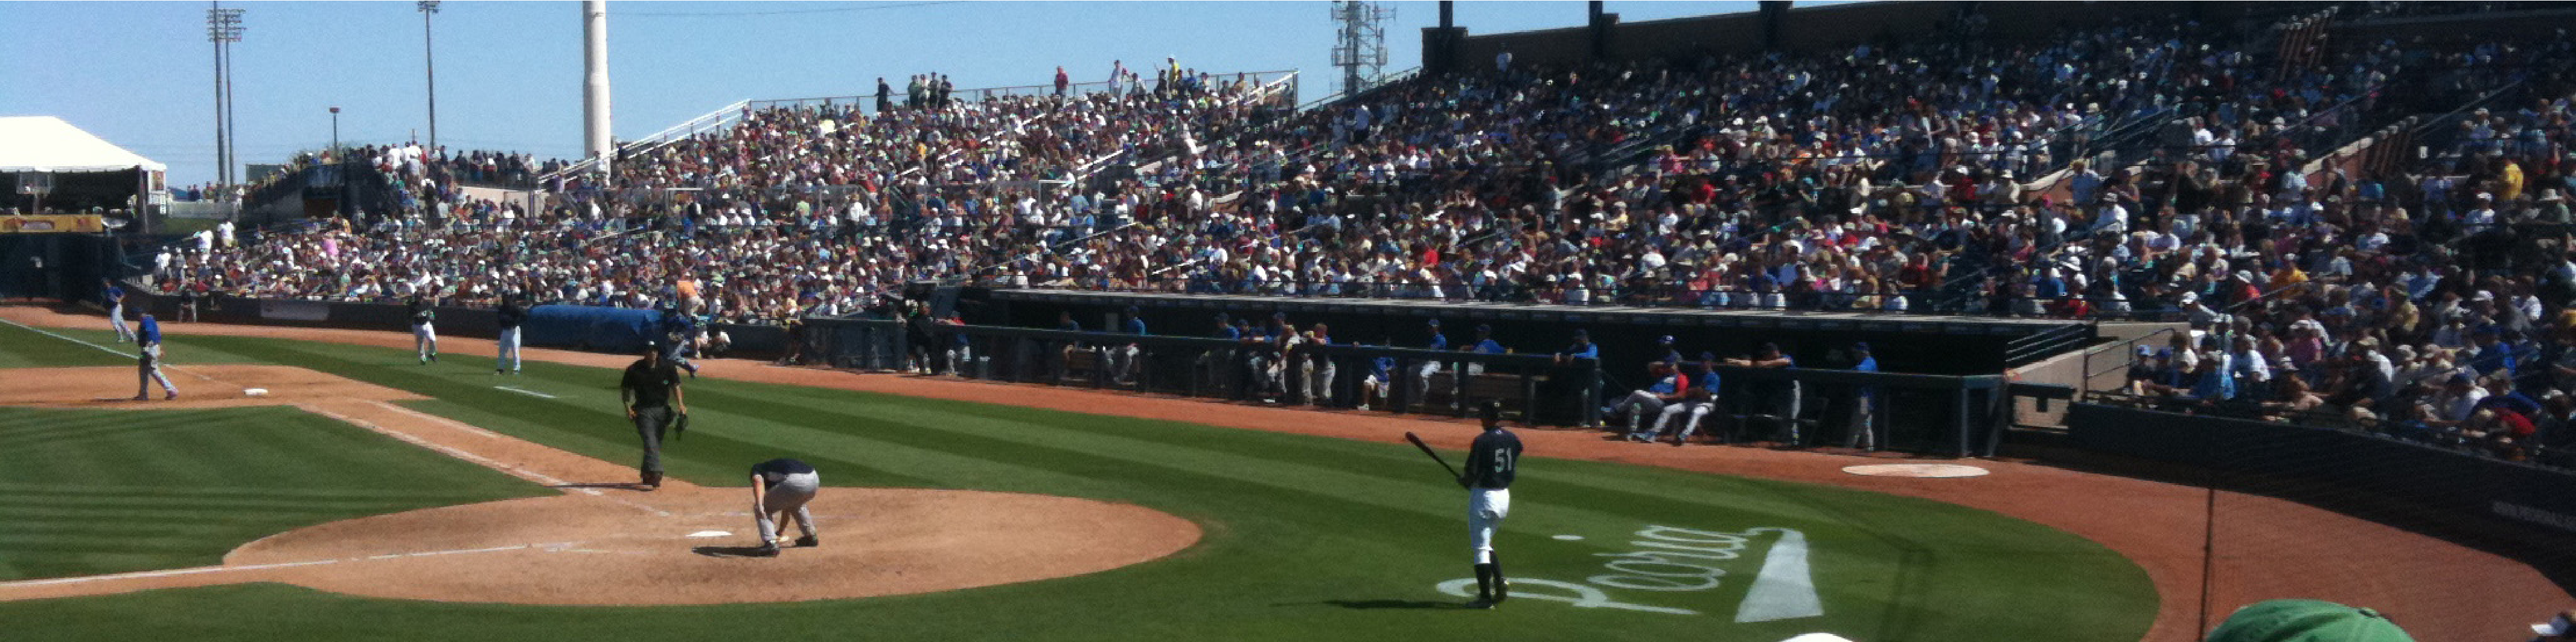
\includegraphics[width=\textwidth]{sampleteaser}
%   \caption{Seattle Mariners at Spring Training, 2010.}
%   \Description{Enjoying the baseball game from the third-base
%   seats. Ichiro Suzuki preparing to bat.}
%   \label{fig:teaser}
% \end{teaserfigure}

\received{20 February 2007}
\received[revised]{12 March 2009}
\received[accepted]{5 June 2009}

%%
%% This command processes the author and affiliation and title
%% information and builds the first part of the formatted document.
\maketitle

\section{Introduction}
Large Language Models (LLMs) have made significant strides in various domains, including natural language processing, machine translation, and text summarization. Among these applications, the use of LLMs for program synthesis and generation has been particularly noteworthy. Projects such as OpenAI's Codex \cite{10.1145/3597503.3639219} and DeepMind's AlphaCode \cite{10.1109/ICSE48619.2023.00181} have demonstrated the impressive ability of LLMs to generate code, showcasing their potential in automating programming tasks. Recent studies have extended this application to programming education. These tools can function as valuable educational assets when implemented responsibly and within appropriate contexts.They can effectively assist various programming tasks including code completion \cite{10.1109/COMPSAC57700.2023.00117}, \cite{10.1145/3639474.3640076}, program repair \cite{10.5555/3618408.3618894}, code explanations \cite{Chen2023GPTutorAC}. The output quality of ChatGPT in these tasks can highly depend on the training data and prompt design \cite{10.5555/3618408.3618894}. 

Building on the growing interest in the use of LLMs for programming education, recent research has evaluated their performance in real-world introductory computer science courses, primarily focusing on assessing the capabilities of current models with existing datasets or previous assignments from students \cite{hicke2023aitaintelligentquestionanswerteaching, anishka2024chatgptplayroleteaching}. For example, Codex can offer immediate feedback on students' programming assignments and produce varied code samples to illustrate programming principles \cite{kumar2024impactguidanceinteractionstrategies}, which reveals that Codex can enhance code generation capability for novice users.

% LLM for LRL as a motivation?
However, the related research concerns particularly commonly used programming languages like Java and Python, which leads to a notable gap in research regarding applying LLMs to statically typed functional programming languages, such as OCaml, which are often used in advanced programming courses. Despite its pedagogical and theoretical importance, OCaml remains underrepresented in programming education research and the datasets used to train LLMs. This limitation also reflects a broader challenge: how to use LLMs to support low-resourced programming languages effectively \cite{mora2024syntheticprogrammingelicitationtexttocode, 10.1145/3689735, deng2024assessingcodegenerationintermediate}. This would support programming education and improve tools and learning materials for a language that plays an important role in teaching functional programming.


This study aims to address this gap by evaluating and comparing LLM performance in the context of OCaml programming education. Specifically, we investigate whether LLMs can solve OCaml programming assignments, effectively repair faulty OCaml code, and testing their performance on theoretical questions included on exams. These theoretical questions assess students' understanding of key functional programming concepts, such as recursion, higher-order functions, and type inference, which are central to mastering the language. The findings from this research will provide insights into the capabilities of LLMs in statically typed functional programming and help compare the performance of different models in this area. Also, we aim to explore how well LLMs handle both practical coding tasks and conceptual questions, offering a more comprehensive evaluation of their utility in an educational setting. This will help identify effective ways for students to use LLMs as learning aids and provide educators with guidance on integrating these tools into OCaml coursework. It will also support the design of programming exercises that promote meaningful learning while reducing the risk of misuse. Finally, our evaluations are critical for enabling researchers to make informed decisions about incorporating LLMs into their courses and guiding students on the optimal and responsible use of LLM-powered tools.



Evaluating LLMs poses several challenges. We often lack knowledge about their training data, raising questions about the reproducibility of results. Additionally, the variability in LLM outputs can lead to inconsistent results, complicating the evaluation process. Moreover, equity and inclusion concerns arise, as the cost of evaluating LLMs may be prohibitive for some reviewers or instructors. Despite these challenges, our research aims to shed light on the practical and conceptual aspects of using LLMs for programming education, particularly in statically typed functional programming languages. By addressing these questions, we hope to contribute to the growing body of knowledge on LLMs and their potential to transform programming education.

\section{Related work}

Large Language Models (LLMs) have emerged as powerful tools in the field of software engineering, particularly in the domains of code generation and repair. These models, trained on vast corpora of code and natural language, have demonstrated remarkable capabilities in understanding and producing programming language syntax and semantics.

Large language models (LLMs) for code generation refer to the use of LLM to generate source code from natural language descriptions, a process also known as a natural-language-to-code task. Typically, these natural language descriptions encompass programming problem statements (or docstrings) and may optionally include some programming context. Code generation has been a long-standing challenge in software engineering. LLMs have shown significant promise in this area, offering the potential to increase developer productivity and assist in rapid prototyping \cite{10.5555/3618408.3618894,wu2024repoformerselectiveretrievalrepositorylevel,DBLP:conf/acl/LuDHGHS22}. For example, LLMs can offer immediate feedback on students' programming assignments and produce varied code samples to illustrate programming principles \cite{kumar2024impactguidanceinteractionstrategies}. An experiment by \cite{10.1145/3545945.3569830} reveals that learners with access to Codex during the training phase performed slightly better on the evaluation. The work by \cite{yetiştiren2023evaluatingcodequalityaiassisted} used the latest versions of ChatGPT, GitHub Copilot, and Amazon CodeWhisperer to generate Python code using the benchmark HumanEval Dataset, and they achieved 65.2\%, 46.3\%, and 31.1\% of the time, respectively. A study by \cite{10.1145/3544548.3580919} investigates how a pedagogically-designed LLM-based chatbot supports students’ debugging efforts in an introductory programming course. Their data revealed that students appreciated the content and experiential knowledge provided by the chatbot, but did not view it as a primary source for learning debugging strategies. 



Similarly, code repair, which involves identifying and correcting errors in existing code, has seen advancements through the application of LLMs. These models can potentially detect both syntactic and semantic errors, suggesting corrections that adhere to best practices and maintain code consistency \cite{DBLP:conf/icse/JiangL021, parasaram2024factselectionproblemllmbased, olausson2024selfrepairsilverbulletcode}. Prenner et al. \cite{10.1145/3524459.3527351} conducted a small-scale evaluation for the Codex model on a simple dataset containing both Java and Python versions of buggy algorithm implementations. Codex is given the buggy function and by using prompt engineering, are then asked to generate a complete fixed function. The results show that Codex is competitive with state-of-the-art learning-based APR tools in Python but worse in Java. In contrast, we show that by using our repair settings, LLMs are able to outperform state-of-the-art APR tools on both Java and Python. Kolak et al. \cite{osti_10340618} also used Codex along with 2 smaller LLMs and evaluated their ability to generate the correct patch line when given the code prefix on the same dataset as the previous work [32]. The evaluation demonstrated the scaling effect of LLMs where the repair results can be improved by using larger models.

The importance of these capabilities extends beyond professional software development into the realm of programming education. LLMs capable of generating and repairing code could serve as powerful educational tools, providing instant feedback to students, assisting in debugging, and offering explanations for complex programming concepts \cite{10.1145/3597503.3639219, 10.1145/3544548.3580919, 10.1145/3631802.3631806, 10.1145/3613904.3642706, jury2024evaluating}. In addition, Kiesler and Schiffner \cite{kiesler2023largelanguagemodelsintroductory} assessed the capabilities of ChatGPT-3.5 and GPT-4 in solving introductory Python programming tasks sourced from CodingBat. Supporting discussions on LLMs’ application in programming education, particularly with development assistants, additional references such as Asare et al. \cite{10.1007/s10664-023-10380-1}, Pearce et al. \cite{DBLP:conf/sp/PearceA0DK22} and Dakhel et al. \cite{DBLP:journals/jss/DakhelMNKDJ23} provide insights into the integration of AI tools within software development environments. These studies collectively underscore the transformative impact of LLMs on programming education, suggesting avenues for future research in optimizing their use for educational enhancement


However, their use also raises important questions about academic integrity and the development of core programming skills.[citations]

\section{Method}

% eval method
% To evaluate how effectively LLMs can fix errors, we conducted experiments using various LLMs in different scenarios: zero-shot and one-shot. In the zero-shot scenario, we provided the LLM with a faulty program and asked it to generate a corrected version without any prior examples. In the one-shot scenario, we first provided the LLM with a faulty program and its corrected version. Then, we presented another similar faulty program and asked the LLM to generate the corrected version.

% We identified similar programs by selecting faulty programs from a student's timeline, considering submissions either earlier or later in the course. This approach helped us evaluate the LLMs' ability to generalize error correction across different contexts.

% For syntax errors, we randomly sampled 500 programs from student submissions, equally distributed among ten homework assignments (HW1-10) from Fall 2022. 


% We also evaluated the LLMs' capability to write complete programs by providing them with 10 different programming assignments and assessing their performance. We measured the pass rate as the percentage of assignments where the LLM generated a correct solution that passed all tests on the first try. Additionally, we evaluated the success rate over multiple attempts (k = 1, 5, 10), recording the number of full grades achieved across these attempts.

% By conducting these evaluations, we aimed to gain insights into the strengths and limitations of different LLMs in both error correction and program generation tasks, particularly in the context of teaching statically typed functional programming languages like OCaml.


Under the subsections below, we elaborate on our methodology. Section 3.1 gives details about how we evaluate LLMs in generating solutions for programming questions, as well as how LLMs perform in repairing the buggy codes selected from student homework. The assignment questions consist of 10 homework from fall 2022. Section 3.2 describes how we classify the conceptual questions chosen from the midterm and final exams into various categories and presents the responses from LLMs for these questions.    


\subsection{Evaluation on programming questions}

% TAs to perform manual grading here
% describe the content of assignment questions
% details of problem description

One of the most popular downstream tasks for code modeling is code generation given a
natural language description. We prompt the model with the same question description as students would see, and ask the models to generate the solution for each programming question with zero-shot learning. Each solution is first graded by the auto-grader, where it is considered correct if it passes all test cases. The maximum grade during the five trials is recorded. Then we also conduct a manual inspection for each solution to check if the style meets our requirements. Typical style issues include not implementing the program tail-recursively, not using HOFs(higher-order functions), or developing imperative language features. We rate the code from 1,2,3 or 4, each corresponding to beginner, developing, proficient, and mastery.

To assess the effectiveness of LLMs in error correction, we conduct experiments in a zero-shot scenario using faulty programs. Here, the LLM is presented with a faulty program with the existing error type and asked to provide a corrected version without prior examples. The faulty programs are sampled from student homework submissions and equally distributed among 10 assignments. Errors in these programs are divided into 3 types based on the compiler message: type error, syntax error, and logical error, where there are 500 programs for each error type (a total of 1500 programs). 

% e.g. binding stack
\subsection{Evaluation on conceptual questions}

To get a better sense of LLMs' ability to understand the underlying logic of functional programming, we also conduct experiments on conceptual questions. In contrast to programming exercises which are designed to build practical skills in implementing concepts through code, conceptual questions typically focus on assessing a student's understanding of fundamental principles and theories, and they often require explanations, proofs, or high-level reasoning. We categorize the conceptual questions from midterm and final exams into five groups: Long answer, Dynamics(evaluations), Type inference, Statics(variable binding, unused variables, substitution/overshadowing), and Induction proof. Following the method described in Section 3.1, we input the model with exam questions and repeat the process 5 times. Here we explicitly specify that the questions are related to OCaml. Additionally, for solutions that require a specific type of structure, we provide an example to guide the model, as it otherwise lacks prior knowledge of the required format. For this part, we also rate the solutions from beginner, developing, proficient, and mastery.


\input{results}
\section{Threats To Validity}
In our evaluation, we assume that the LLMs are already fully trained and that no additional re-training or learning occurs during the evaluation process. This assumption is crucial because it impacts the validity and reproducibility of our results. If any form of additional learning were to take place during the evaluation, it could skew the outcomes and lead to an overestimation of the LLMs' capabilities.

Furthermore, the variability in LLM outputs poses a challenge to the consistency of our findings. Since LLMs can produce different results given the same input on different occasions, this variability must be accounted for in our analysis. We mitigate this by averaging results over multiple runs, but inherent unpredictability remains a concern.

Another threat to validation arises from the unknown nature of the training data used to develop the LLMs. Without detailed knowledge of the datasets and the specific programming tasks the LLMs were exposed to during training, it is difficult to ascertain whether the models have been inadvertently trained on similar tasks or even specific examples present in our evaluation dataset. This could result in biased performance metrics that do not accurately reflect the models' generalization capabilities.

Additionally, the evaluation process itself could introduce biases. For example, the selection of faulty programs and the criteria for what constitutes a "similar" program may affect the outcomes. We have attempted to mitigate this by using a random sampling approach and defining clear criteria for similarity, but subjective decisions are unavoidable.

The cost and accessibility of running extensive evaluations with LLMs also present equity and inclusion concerns. Not all researchers or educators may have the resources to replicate our study, which could limit the generalizability and applicability of our findings across different contexts.











\section{Appendices}

If your work needs an appendix, add it before the
``\verb|\end{document}|'' command at the conclusion of your source
document.

Start the appendix with the ``\verb|appendix|'' command:
\begin{verbatim}
  \appendix
\end{verbatim}
and note that in the appendix, sections are lettered, not
numbered. This document has two appendices, demonstrating the section
and subsection identification method.


%%
%% The next two lines define the bibliography style to be used, and
%% the bibliography file.
\bibliographystyle{ACM-Reference-Format}
\bibliography{sample-base}


%%
%% If your work has an appendix, this is the place to put it.
\appendix


\end{document}
\endinput
%%
%% End of file `sample-sigconf-authordraft.tex'.

%%% Local Variables:
%%% mode: latex
%%% TeX-master: t
%%% End:
